\documentclass[a4paper, 11pt, onecolumn]{article} % A4 paper and 11pt font size
\usepackage[top=2.5cm, bottom=2.5cm, left=2.5cm, right=2.5cm]{geometry}

\usepackage[pdftex]{graphicx}
\usepackage{hyperref}
\usepackage{multirow}
%\usepackage{fourier} % Use the Adobe Utopia font for the document - comment this line to return to the LaTeX default
\usepackage{mathptmx}
%\usepackage[english]{babel} % English language/hyphenation
\usepackage{amsmath,amsfonts,amsthm} % Math packages
\usepackage{sectsty} % Allows customizing section commands

\bibliographystyle{plain}

\allsectionsfont{\normalfont\scshape} % Make all sections centered, the default font and small caps

\usepackage{fancyhdr} % Custom headers and footers
%\pagestyle{fancy}
\rhead{ }
\renewcommand{\headrulewidth}{0pt} % Remove header underlines
\renewcommand{\footrulewidth}{0pt} % Remove footer underlines
\setlength{\headheight}{13.6pt} % Customize the height of the header

\numberwithin{equation}{section} % Number equations within sections (i.e. 1.1, 1.2, 2.1, 2.2 instead of 1, 2, 3, 4)
\numberwithin{figure}{section} % Number figures within sections (i.e. 1.1, 1.2, 2.1, 2.2 instead of 1, 2, 3, 4)
\numberwithin{table}{section} % Number tables within sections (i.e. 1.1, 1.2, 2.1, 2.2 instead of 1, 2, 3, 4)

\setlength\parindent{0pt} % Removes all indentation from paragraphs - comment this line for an assignment with lots of text
\setlength\parskip{0.5em}

\setlength\columnsep{18pt}

\title{
	\vspace{-3.0cm}
	\horrule{0.4pt} \\[0.2cm] % Top horizontal rule
	\vspace{0.2cm}
	\Large ART-CG: Assisted Real-time Content Generation of 3D Geometry through Machine Learning\\
	\horrule{0.4pt} \\[0cm] % Bottom horizontal rule
	\vspace{-0.5cm}
}
\date{} % No date

\newcommand{\horrule}[1]{\rule{\linewidth}{#1}} % Create horizontal rule command with 1 argument of height

%%%%% FOOTNOTE EXAMPLE %%%%%
%\footnote{\href{www.google.com}{www.google.com}}


\begin{document}
\maketitle
\thispagestyle{fancy} % Show header on front page
%\pagestyle{plain} % Remove header on following pages

\section*{The Proposers}
\hrule\vspace{0.5em}
\subsection*{The University of Bristol}
The University of Bristol is a leading research institution and a member of the Russell Group. Its Department of Computer Science has pioneering research groups in cryptography, robotics, interaction and graphics, theory and algorithms, intelligent systems, computer vision, and microelectronics. 
The university is the largest independent employer in Bristol, generating a total income of \textsterling 566 million (of which \textsterling 146 million were from research grants and contracts). Its sponsors include EPSRC, ESRC, AHRC, SSRC, and many industrial partners.

\textbf{Dr D. K. Diep} is a core member of the Intelligent Systems research group in the Department of Computer Science at the University of Bristol. He has recently conducted a research project on the application of machine learning to hair geometry. His past collaborations with ManualDesk and Circle Enix in research of learning-based solutions for 3D asset production has been adopted by leading firms to develop cutting-edge, state of the art tools and applications.

\textbf{Dr C. H. Ek} is a Professor of Computer Science at the University of Bristol. His research specialises in multi-view latent variable models in machine learning. Dr C. H. Ek currently contributes to machine learning research projects in collaboration with Prof N. D. Lawrence and Dr A. Damianou at Amazon Research Cambridge, as well as Dr N. Campbell at the University of Bath.

\subsection*{ManualDesk, Inc.}
ManualDesk is a UK-based software corporation that specialises in the 3D production pipeline. Its technology is the industry standard for the engineering, manufacturing, architecture, and entertainment industries. In 2014, ManualDesk employed over 5,000 and its total assets were estimated to be worth \textsterling 1.6 billion. Open3DML is an initiative for developing open-source solutions that apply machine learning to 3D production led by ManualDesk. 

\textbf{Dr D. Hu} was a technical artist for 15 years before joining ManualDesk as an industrial researcher for innovative 3D production tools. Seven years later, she is currently the research director of ManualDesk. Since then, she has overseen over twenty research projects in the department and participated in over thirty funded research projects.

\subsection*{Circle Enix, Ltd.}
Circle Enix is a UK-based video game development studio and publisher. It owns a research department that employs cutting-edge technology to improve the user experience of consumers. In 2015, Circle Enix employed over 450 and its total assets were estimated to be worth \textsterling 56 million. 

\textbf{Dr C. Strife} has over 30 years of experience in developing real-time graphical systems and was the lead programmer in Circle Enix before becoming the research lead.

\newpage

\section*{Case for Support}
\hrule\vspace{0.5em}
\section{Overview and Motivation}
\label{motivation}
%%% Background & Hypothesis %%%
The production of 3D assets is a meticulous and time-consuming procedure that also requires expert knowledge. Content developers create, manipulate, and maintain high-dimensional 3D geometric data ranging from an order of thousands to millions of data points. State of the art 3D software offers an extraordinary number of features to tackle the complexity of 3D production. However, this promotes a steep learning curve and builds a high barrier to entry for non-experts to produce 3D content. Our proposition of assisted real-time content generation investigates simplification of 3D asset production through application of machine learning.

%%% National Importance %%%
Application of 3D assets contributes immensely to the general public.
Computer-aided-design (CAD) drives engineering and manufacturing.
Computer-generated imagery (CGI) supports the entertainment industry.
The field of medicine has utilised 3D printing, and its application is projected to expand \cite{3dprinting}.
Visualisation, simulation and research often make use 3D assets \cite{simulation}.
Computer graphics (CG) is not only extensively applied, according to \textit{John Peddie Research (JPR)}, the CG market itself will exceed \$235 billion by 2018 \cite{cgmarket}.

%%% Challenges %%%
Definition of geometric representations is often by describing visual properties. For example, polygonal meshes are formed from \textit{edges}, \textit{vertices},  and \textit{faces}. While such approach is sensible for traditional use, the resulting data will have varying dimensionality. This misalignment of dimensionality is problematic for machine learning methods that require computational evaluation and comparison. Creative content is sensitive to corruption, minor changes to a component can be sufficient to invalidate an entire object as a whole. Thus, conventional feature extraction methods are not applicable to 3D geometric data.

The \textit{topology} of a surface is the arrangement of components. The topological structure has practical consequences on the performance of a 3D Topology determines the rendering efficiency and behaviour in reaction to algorithmic operations. Incorporating the idea of topology creates an ambiguous many-to-one mapping of geometric data to the true surface it represents. This ambiguous aspect of geometric representation again contributes to the difficulty of applying established learning methods.

Traditional learning-based approaches generalise a solution by training with a large data set. Unfortunately, 3D data is not as easily attainable when compared to other mediums such as images. Despite the abundance of exemplary 3D output produced, most are not available to the public. Freely available 3D content vary in stylistic properties and suffer from the lack of quality control. In practice, the pool of available 3D exemplars is small. The learning model applied must be robust with small training sets, imperfect examples, and the presence of uncertainty.

The subjective nature of evaluating artistic products poses a problem for computational solutions. A creative environment demands versatility. This incertitude aspect necessitates learning a regression model that can predict a set of acceptable solutions as an assisting procedure, as opposed to a fully-automated process.

%%% Research hypothesis and objectives %%% 
A learning-based perspective towards production can reuse exemplary data available to automate the task at hand.
Identifying commonly recurring properties remove the need to complete repetitive operations manually, leading to \textit{simplification} of the production pipeline. Non-experts receive the ability to create 3D assets, allowing focus on the human aspect of design without requiring to learn the intrinsics of 3D software. 
A real-time method that uses exemplary data as a reference gives rise to the idea of \textit{rapid prototyping}. Typically, visualising a concept is presented through a medium that is faster to produce, such as conceptual art or blueprint sketches. Such practice is common but risks misrepresentation from translation between mediums. Exposing a fast method of sampling from a latent space learned from exemplary designs can provide initial geometry to be refined and presents a clearer indication of a concept.

Assisted real-time content generation extends the utility of machine learning research for the creative field. Past research has used probabilistic nonlinear dimensionality reduction to learn a \textit{latent space} (low-dimensional representation) from a high-dimensional space, simplifying data by reducing the number of variables needed to be considered. Such an approach has been employed for animation \cite{styleik}, basic drawings \cite{latentdoodle}, font design \cite{fontmanifold}, and virtual hair modelling \cite{artcg}. ART-CG builds upon the foundation of learning-based solutions for creative purposes established and transfers it to complex, enormously high dimensional 3D geometric data by resolving the challenges outlined.


\section{Programme and Methodology}
\subsection*{Work Package 1 (WP1): Parametrisation of 3D Objects}
\textbf{Research Leader:} Dr D. K. Diep\par

The principal research objective of this work package is to establish an intermediate standardised 3D representation suitable for machine learning. As outlined in section \ref{motivation}, conventional feature extraction methods are insufficient to represent delicate details of surfaces. WP1 investigates methods of approximating object successfully so that the aligned data are comparable and minimises the data loss from approximation.

Geometric representations can describe arbitrary surfaces, adjusting to the need of a content creator flexibly. The unusual surface output is undesirable for the purpose of assisted content generation. Placing constraints on the space of possible surfaces described can ensure a level of quality. In computer graphics, there exists procedural generative methods that synthesise complex geometry from a smaller set of input parameters.

The first objective of this phase is to evaluate current generative models available as candidates that can be intermediate representations for machine learning methods. The industrial standard for CGI predominately uses mesh models, a high-fidelity representation but is susceptible to noise corruption - marginal alteration on the vertices of a mesh model can change its appearance significantly. Generative models and representations of surfaces is a significant sub-topic with much to explore. Potential intermediate representations include generalised cylinders, voxels, shape histograms, and 3D salient points \cite{salientpoints}. It is critical for the generalised model to strike a balance between the cardinality of inputs required and the fidelity it can capture.

From the set of existing models, we will formulate an extended model such that it contains a comparable metric and preserves the necessary properties of geometric data including preservation of the topology. Finally, we devise sampling methods to acquire an approximation of a 3D asset by accurately estimating the inputs of a generative model.

\subsubsection*{Deliverables} 
\begin{enumerate}
	\item \textbf{D1a.} Investigate techniques or generative model(s) that is suitable for resolving the alignment problem of raw input data, allowing a sufficient approximation of generative parameters with the same dimension.
	\item \textbf{D1b.} Formulate techniques or generative model(s) that preserve geometric properties to maintain an organised topology desirable for 3D assets.
	\item \textbf{D1c.} Devise methods to sample generative inputs from approximating a 3D asset to the closest equivalent defined in a generative model.
\end{enumerate}

\subsection*{Work Package 2 (WP2): Learning a Regression Model of 3D Objects}
\textbf{Research Leader:} Dr C. H. Ek\par

The research objective of this phase is to investigate methods that are ideal for learning the generation of 3D objects. There are many machine learning models that can be used for regression. A model that is fitting for production of 3D assets must address the following:
\begin{itemize}
	\item Subjective evaluation of artistic products.
	\item Small training data sets.
	\item Missing information and uncertainty.
\end{itemize}

Past research has utilised the Gaussian process latent variable model (GP-LVM) to learn a probabilistic nonlinear latent manifold embedding of the observed data. The GP-LVM model is a strong contender as a regression model for the ART-CG framework as a probabilistic solution can offer multiple acceptable predictions for a content creator to choose from \cite{gplvm}. Gaussian processes are non-parametric; thus, it can flexibly capture a range of possible values fitting for general 3D assets. Chai et al. (2016) employed a neural network as part of a system that produces 3D hair geometry \cite{autohair}. The scope of investigation encapsulates comparison of different regression models available.

The complexity of 3D geometry calls for advanced regression models. Extending models with concepts such as layering hierarchy or applying deep learning \cite{deepgp} are viable approaches. Considerations include the limitations of learning models, evaluating the trend of performance as training data set scales. Online (continually) learning models update with new observations without requiring retraining; this approach is a possible solution for refining regression models even with an initially small training set.

\subsubsection*{Deliverables} 
\begin{enumerate}
	\item \textbf{D2a.} Investigate viable learning models that are suitable for generation of 3D objects.
	\item \textbf{D2b.} Applying research of complex models such as hierarchical layering, deep learning, and online training to utilise an advanced regression model for complex 3D geometry.
	\item \textbf{D2c.} Assorting competitive kernels that establish effective default prior probability distributions suitable for 3D geometry regression models and learning hyperparameters.
\end{enumerate}

\subsection*{Work Package 3 (WP3): Generation and Reparation}
\textbf{Research Leader:} Dr D. K. Diep\par

Prediction by regression models contains a level of uncertainty. In the context of 3D assets, some scenarios outline specific constraints for geometry. An example would be hair object that should not grow inwards into a scalp surface. Engineering design and architecture also apply strict limitations. This phase investigates methods of generation that conform with specified constraints, performing reparations appropriately so that the output is optimised and practical. 

Applying constraints within the regression model can be achieved through weighting inputs or implementing a cost function that penalises undesirable attributes.  Post-prediction reparation would consider regulating output through heuristics or physical simulation to remove overlapping surfaces and similar properties.

\textbf{Deliverables}
\begin{enumerate}
	\item \textbf{D3a.} Investigate and formulate methods that constrain the regression model.
	\item \textbf{D3b.} Investigate and formulate methods that repair the output of a regression model.
\end{enumerate}

\subsection*{Work Package 4 (WP4): High-Fidelity Generalised Parametrisation}
\textbf{Research Leader:} Dr C. Strife\par

Techniques such as vector displacement maps provide an additional layer of detail for 3D assets. This phase looks into incorporating displacement maps and similar methodologies as a part of the ART-CG framework to improve the quality of predictions by the regression model without sacrificing topology.

\subsubsection*{Deliverables} 
\begin{enumerate}
	\item \textbf{D4a.} Learning an additional model of high-fidelity generalised parametrisation to modify 3D assets.
	\item \textbf{D4b.} Incorporating high-fidelity generalised parametrisation as part of the generative model for the 3D geometry regression model.
\end{enumerate}

\subsection*{Work Package 5 (WP5): Intuitive Presentation of Latent Control Variables}
\textbf{Research Leader:} Dr D. Hu\par

Simplifying the production process through learning a regression model delegates control from the observed variables to descriptive latent (unobserved) variables that are input to the regression model. Determining the output with latent variables reduce the number of inputs required, but a solution is of no use if it is counter-intuitive or difficult to use effectively. Latent variables computed are not well-described, there are no labels that associate the variables with a semantic context. This phase aims to deliver an intuitive presentation for latent control variables and methods that help to convey the semantic meaning of latent variables.


\subsubsection*{Deliverables} 
\begin{enumerate}
	\item \textbf{D5a.} Evaluating and devising methods of associating latent control variables to semantic properties.
	\item \textbf{D5a.} Presenting latent control variables intuitively.
\end{enumerate}

\subsection*{Work Package 6 (WP6): Impact and Success Strategy}
\textbf{Research Leader:} Dr D. K. Diep\par

Dr D. K. Diep and Dr C. H. Ek as the principal investigator and co-investigator respectively will maximise the chance of success by managing the team contributing to the research project. Regular weekly meetings will be held by members of the research lab with the post-doctoral researchers and PhD students to ensure that the team remains on track and progressing smoothly. Monthly reports are to be produced regarding work completed. Quarterly meetings with industrial partners will be held to stay in touch and discuss project progression.

The team will contribute to the field of machine learning and computer graphics research by attending conferences. The exchange of ideas with other researchers will be mutually beneficial and bring attention to the ART-CG initiative. Supplementary workshops will illustrate the capability of the ART-CG framework through prototype implementations and discuss potential research areas that are worthy of exploring.

\subsubsection*{Deliverables} 
\begin{enumerate}
	\item \textbf{D6a.} Monthly reports regarding updates on progress.
	\item \textbf{D6b.} Recorded minutes of weekly meetings with post-doctoral researchers and PhD students.
	\item \textbf{D6c.} Recorded minutes of quarterly meetings with industrial partners (Circle Enix and ManualLab).
	\item \textbf{D6d.} Evaluation of strategies employed during project execution.
	\item \textbf{D6d.} Publicising ART-CG through conferences and workshops.
\end{enumerate}

%\newpage

\bibliography{research_proposal}

\newpage

\section*{Budget}
\hrule\vspace{0.5em}

\begin{table}[!h]
	\centering
	{\renewcommand{\arraystretch}{1.8} %<- modify value to alter spacing
	\begin{tabular}{|l|c|c|c|}
		\hline
		Item		& Quantity	& Annual cost per unit (\textsterling)	& Total cost over duration (\textsterling)\\
		\hline
		PI			& 1			& 100,000				& 300,000\\
		\hline
		CoI			& 1			& 75,000				& 210,000\\
		\hline
		PD			& 2			& 50,000				& 300,000\\
		\hline
		PhD			& 2			& 20,000				& 120,000\\
		\hline
		Technical Artist (10\%) & 1 & 10,000			& 30,000\\
		\hline
		Workstation	& 2			& 500					& 1,000\\		
		\hline
		Workshop	& 2			& 1,000					& 2,000\\		
		\hline
		Conference	& 3			& 6,000					& 18,000\\		
		\hline
		Travel \& accommodation & X	& 5,000				& 15,000\\		
		\hline
		Training Data& X		& X						& 150\\
		\hline
	\end{tabular}
	}
	%\caption{budget}
\end{table}

\vspace{1cm}

\textbf{Total cost:} \textsterling 996,150.00

\newpage

\section*{Justification for Resources}
\hrule\vspace{0.5em}

The principal investigator (PI) and co-investigator (CoI) oversees scheduling, administration, and execution of the research project such that it successfully achieves the deliverables promised.
The principal investigator, Dr D. Diep, is the instigator of the research proposal and will be the one with ultimate responsibility for directing the project in the right direction.
The co-investigator, Dr C. H. Ek, will support and assist the principal instigator in leading the research project.
The investigators will ensure that the project is executed in compliance with governing laws and regulations, as well as adhering to the policies outlined by sponsors.

Post-doctoral researchers bring expertise knowledge from related fields that will assist in making informed decisions to carry out research efficiently. PhD students will support the development of the research project and acquire skills from the area of machine learning, such as probabilistic non-linear dimensionality reduction and other significant learning-based models applicable to the 3D production pipeline.

A part-time technical artist will create and modify geometric data to incorporate extreme or specific test cases considered by the project. Purchasing an initial training set is more efficient than commissioning a professional artist. However, as the project develops, the input of a professional artist will be required to introduce ART-CG to the production pipeline successfully.

Circle Enix and ManualLab will contribute with their technical expertise for this project. Exchanging ideas create synergy between academia and industry to improve the chance of delivering successful results.

Two shared workstations in office will process the data and prototyping ideas. While each member of staff is expected to own a personal machine, the workstations will act as a central point for development. Circle Enix has agreed to offer their cloud computing resources as well as access to their render farm facility for this project.

The purpose of conferences and communication is to stay up to date with the latest state of the art research and spreading awareness of our research project. The budget includes national and international travel and accommodation costs. Publicity for the initiative will encourage adoption and draw in potential opportunities for collaboration. Exchanging findings with other researchers will be beneficial for all projects within the community.

\newpage

\section*{Impact Statement}
\hrule\vspace{0.5em}

The ART-CG project aspires to impact by simplification of the 3D production pipeline, supplying the growing demand for 3D assets. As mentioned in section \ref{motivation}, the production of 3D assets plays a pivotal role in business, engineering, and entertainment. It is an industry predicted to be worth \$ 235 billion in 2018. The research project will impact on three key beneficiaries: academics of machine learning for creative purposes, 3D artists and designers, businesses that work with 3D assets, and consumers that benefit from the production of 3D assets.

ART-CG brings together two monolithic subjects of computer science: machine learning and graphics. Focusing on effective methods for the production pipeline bring economic and cultural motivation for further research. Academics will incorporate topology-preserving machine learning methods designed to be adaptable for enormously high-dimensional and delicate data. State of the art geometric processing and generating techniques will be re-evaluated to comply with a learning-based perspective. Studying the user experience for revolutionary tools that make use of latent unobserved control variables will improve presentation and ease of use. ART-CG will contribute to the field of machine learning for content creation through academic publications and prototypes that provide insights into its capabilities and limitations.

The research department of ManualDesk is interested in methods of effectively presenting a low-dimensional representation acquired from dimensionality reduction such that content creators would find intuitive to use.
ManualLab is looking to revolutionise the way of producing 3D assets by delegating much of the manual work to be automated by learning-based tools. The methodology introduced in ART-CG is to be incorporated into the \textit{intelligent systems} expansion for their industry-leading open-source 3D software, \textit{ManualLab Mixer} as part of the Open3DML initiative. Implementations based on the ART-CG framework will impact on individual content creators such as artists and designers, which in turn makes an impact on businesses that require 3D assets for operation.

% The collaborative effort between University of Bristol with industrial leaders ManualLab and Circle Enix seek to research effective machine learning methods and frameworks for simplification of the production pipeline.

Circle Enix is seeking to apply assisted content creation tools for non-expert consumers to create custom assets for their upcoming next-generation video game software, \textit{Final Craft}. Applications that allow users to create their personal content could integrate the ART-CG framework to prevent inappropriate or undesirable creation from being produced while providing options that surpass existing alternatives. A space of reasonable options generated from predefined outputs by the developers will allow users to interpolate between sensible configurations, providing an excellent level of customisation while adhering to defined constraints. 

The advent of virtual reality, augmented reality, and 3D printing prompts for a method of enabling non-experts to create personal 3D content. Utilisation of ART-CG for rapid prototyping of prosthetics and artificial organs for 3D printing in medical applications saves lives and improve living standards. Solutions covered in this project will be in line with the massive push for 3D-oriented consumer updates, such as the \textit{creators update} for Windows 10 from Microsoft. Consumers will be able to enjoy an improved quality of 3D assets and obtain the ability to produce personal content even without expertise in 3D production.

WP5 focuses on establishing the pathway to impact. Research progress documented in frequent reports will record methodology and evaluate the effectiveness of strategies employed. Regular meetings will ensure that the project is making progress and prepare to adapt to new-found problems discovered over the duration of the ART-CG project. Attending conferences during the project and then holding workshops near the end of the project engages with the community to prompt for further investigation.

\newpage

\section*{Work Plan}
\hrule\vspace{0.5em}

\begin{figure}[!h]
	\centering
	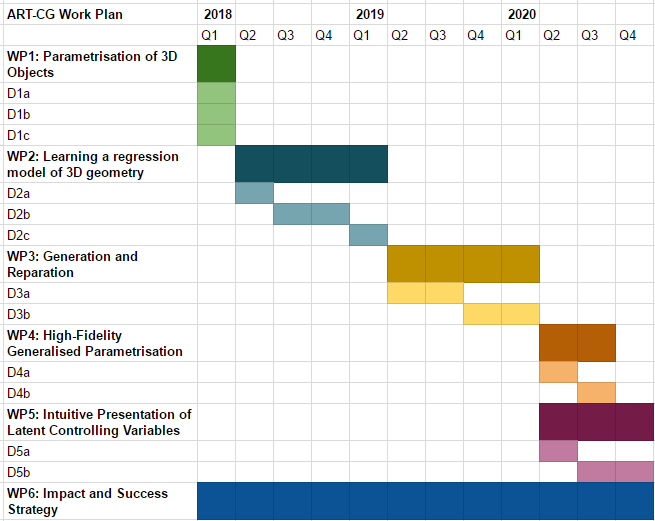
\includegraphics[scale=1.0]{images/workplan}\\
\end{figure}

\end{document}